%
% File: chap05.tex
% Author: Antigoni Kourou
% Description: Evaluation
%


\let\textcircled=\pgftextcircled
\chapter{Evaluation}
\label{chap:eva}

\initial{F}or checking the efficiency of the proposed pipeline, its performance is compared to ratings given by humans for two main purposes. First, the evaluation aims to find out how well VADER, the selected sentiment detector, performs in the chosen dataset and secondly, how well can the pipeline identify the features of a certain sentence of review. To answer these two questions, a sample of 100 sentences are randomly chosen from the dataset and are given to humans for rating. Each respondent is required to first read the sentences, then to estimate a score of sentiment for each of them on a scale from -1 to +1. In a second task, thes respondents are asked to mark which of the six accommodation features does the sentence refer to. These tasks are similar to what the pipeline is programmed to do. 
% Evaluation form in Appendix 
The evaluation form is completed by 5 humans, who come from different educational backgrounds, are geographically diverse and are Airbnb users. Their answers are analyzed and compared to the pipeline output using SPSS. Considering the diversity between users, their evaluations are firstly compared to each other using correlation values between samples and distribution statistics. This analysis showed that three of the respondents had very similar answers, consisting in a correlation varying between 72\% to 83 \% between each other and a very similar distribution curve. 
%These output of the analysis in SPSS can be found in Appendix. 
Based on these results, the chosen sample to represent the human ratings are the evaluations of the three "high quality" respondents.

\section{Evaluation of VADER algorithm}

To check the performance of VADER in the dataset, first the mean scores of the three respondents per each sentence are calculated. These mean scores represent the actual rating values, thus VADER scores would  be the predicted values.  For measuring the differences between them, the chosen method is Root Mean Square Error (RMSE).
\begin{equation}
 RMSE \equiv^{def} \sqrt {{\frac{{\sum\limits_{{i = 1}}^{100} {{{\left( {{y_\textsubscript{i (Humans)}} - {{\hat{y}}_\textsubscript{i (VADER)}}} \right)}^2}} }}{{100}}}}
 \label{RMSE}
\end{equation}
The RMSE between the two samples results to be 0.487, meaning that the VADER is not the perfect predictor of human ratings but considering that the Standard Error of Mean (SEM) in differences is 0.0489, we can conclude that there is no tendency of VADER to under-estimate or over-estimate the human ratings. From Figure \ref{fig:distribution} can be noticed that the two datasets share the same mean (4.125 compared to 4.13), the same median and mode (both equal to 4.5) and have similar standard deviations. 
\begin{figure}[h!]
	\centering
	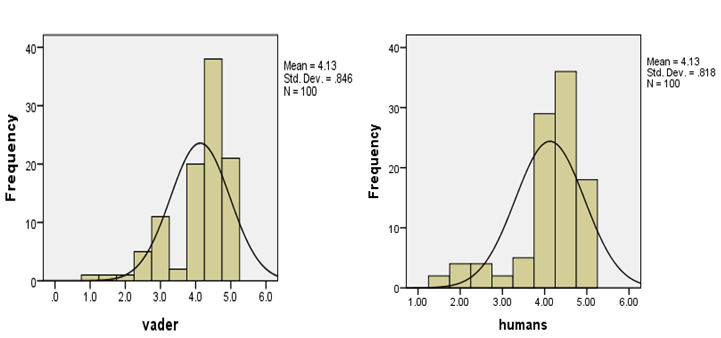
\includegraphics[height=0.33\textheight]{graphs_vader_humans}
	\caption{Distribution of VADER and humans' sentiment scores}
	\label{fig:distribution}
\end{figure}

The differences between VADER scores and human ratings result in 60\% of cases when VADER has detected the exact score as human logic, 24\% cases where the difference is just half a star, 14\% cases with one star difference and the 2\% cases with more than one star difference. The highest value of error is 1.5 stars, which means that VADER will never consider a very positive sentence as a very negative one and the other way round. However, it may consider these kind of sentences as neutrals or may be confused of the sign of sentences with slight sentiment.

\section{Evaluation of feature identification}
The effectiveness of the proposed technique for feature identification is measured by using precision, recall and accuracy as suggested by \cite{huang2006performance}.
The existence of a feature in a sentence is true when it is identified by the majority of respondents. Therefore for each \todo{changed the whole explanation here as suggested} feature, TP (true positives) is the number of sentences that the algorithm correctly identifies the feature, FP (false positives) is the number of sentences that the algorithm falsely identifies the feature; FN (false negatives) is the number of sentences that the algorithm fails to identify it and TN (true negatives) is the number of sentences that the algorithm correctly doesn't identify the feature. The formulas for calucating the precision, recall and accuracy of each feature are:
\begin{align}
Precision  (p) =\frac{TP}{TP+FP} \hspace{1cm}
Recall  (r) = \frac{TP}{TP + FN} \hspace{1cm}
Accuracy (a) = \frac{TP + TN}{TP+TN+FP+FN}
\end{align}
In other words, \textit{accuracy} refers to the quality of correct judgment of the algorithm about a feature.  \textit{Precision} refers to correctness in cases where feature is identified, and recall shows the portion of sentences that the pipeline fails to identify the feature. Ideally the algorithm shall have values of precision and recall close to 1 for each of the features.
These values for each feature are illustrated in Figure \ref{fig:matrix}, which shows that the algorithm manages to identify some features better than others. For example the \textit{value} and \textit{cleanliness} features of the listing are identified almost always with high precision and recall, but a low precision for \textit{communication} means that the algorithm retrieves many FP. The opposite happens for \textit{check in} when the precision is very high but many sentences fail to be identified. In average for the six features, the algorithm reaches the accuracy and precision 77.8\% and recall 79.2\%. Future work needs to be done in improving this step of the pipeline.
\begin{figure}[h!]
	\centering
	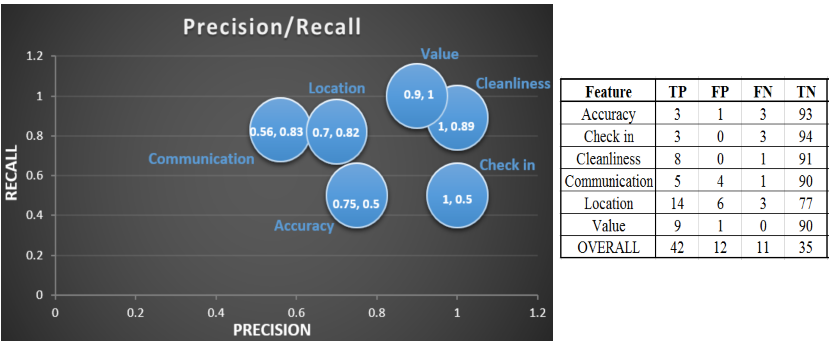
\includegraphics[height=0.3\textheight]{PR_table}
	\caption{Precision/Recall matrix for feature identification}
	\label{fig:matrix}
\end{figure}